% ICASSP paper — NPU-friendly LiSenNet.
% Template: ICASSP author kit (spconf.sty + IEEEbib.bst, vendored).
% NOTE: check the target year's anonymity policy before submission; the author
% block below is NOT anonymized.
\documentclass{article}
\usepackage{spconf,amsmath,graphicx}
\usepackage{booktabs}
\usepackage{xcolor}
\usepackage{url}

% Red bold TODO marker for everything still to be filled in.
\newcommand{\todo}[1]{\textbf{\textcolor{red}{[TODO: #1]}}}

\graphicspath{{figures/}}

% ---------------------------------------------------------------------------
% Title candidates (pick one):
%  (a) the one below;
%  (b) "From GRUs to the NPU: A Deployment-Hardened LiSenNet for
%       Microcontroller Speech Enhancement";
%  (c) "LiSenNet on a Milliwatt NPU: Hardware-Aware Redesign, Quantization,
%       and Frame-Level Streaming".
% ---------------------------------------------------------------------------
\title{Rethinking LiSenNet for Microcontroller NPUs:\\
       Hardware-Aware Redesign, Quantization, and On-Device Streaming}

\name{Cl\'ement Laroche \todo{co-authors}\thanks{\todo{Acknowledge the EU
NeAIxt project / funding as appropriate. Check the ICASSP anonymity policy of
the target year before adding names.}}}
\address{\todo{Affiliation(s)}}

\begin{document}
\ninept
\maketitle

% ===========================================================================
\begin{abstract}
Lightweight speech-enhancement models are designed for real-time CPU
inference, but the emerging class of microcontroller NPUs accelerates only a
narrow, integer-quantized operator vocabulary --- typically excluding the
recurrent layers and normalizations these models rely on. We take LiSenNet, a
37\,k-parameter sub-band dual-path enhancer, as a case study and redesign it
for the STM32N6 Neural-ART accelerator. We (i) replace the dual-path GRU
bottleneck with an equally accurate dual-path \emph{convolutional} one,
(ii) harden every primitive for int8 hardware (BatchNorm folding, bounded
ReLU6 activations, transposed-convolution upsampling), and (iii) show that
post-training-quantization loss concentrates in the model's \emph{decoder},
which activation clipping and a two-recipe quantization scheme largely
recover. The result matches the GRU reference in FP32 (PESQ 3.084 vs.\ 3.006
on VoiceBank-DEMAND) and surpasses it after quantization (3.014 all-int8
vs.\ 2.930). On silicon, the deployed model streams \emph{frame-by-frame} at
4.83\,ms per 16\,ms frame (real-time factor 0.30) with one-hop algorithmic
latency and PESQ 3.013 --- the highest-quality real-time streaming enhancer
we measure on this NPU class. Deploying all six hardened variants also settles
two design questions empirically: the float-decoder recipe that scores highest
offline (3.052) is \emph{not} deployable (34\,ms/frame), and a stateless graph
that recomputes the receptive field every frame --- although it uses the
accelerator $6\text{--}8\times$ more efficiently than the stateful one --- is
$12\text{--}26\times$ slower, because it pays a $70\text{--}200\times$
recompute. Explicit streaming state, not recompute, is what makes this class
of model real-time.
\end{abstract}

\begin{keywords}
speech enhancement, edge AI, neural processing unit, quantization, real-time
streaming
\end{keywords}

% ===========================================================================
\section{Introduction}
\label{sec:intro}

Single-channel speech enhancement (SE) has reached remarkable quality at tiny
parameter budgets: models such as RNNoise~\cite{valin2018rnnoise},
NSNet2~\cite{braun2020nsnet2}, DeepFilterNet~\cite{schroter2022deepfilternet}
and LiSenNet~\cite{yan2024lisennet} run in real time on a single CPU thread.
Meanwhile, microcontrollers are acquiring dedicated neural accelerators ---
e.g.\ the Arm Ethos-U family and ST's Neural-ART --- that promise an order of
magnitude better energy per inference than the host core. These NPUs,
however, accelerate a narrow operator vocabulary: int8 convolutions and
matrix multiplies with a fixed set of layout, kernel and normalization
constraints. The recurrent layers, multi-axis LayerNorms, and parametric
activations that lightweight SE models favor either fail to compile or fall
back to the microcontroller core, forfeiting the accelerator.

This paper asks what it actually takes to move a state-of-the-art
lightweight enhancer onto such an accelerator \emph{without giving up
quality}. Using LiSenNet~\cite{yan2024lisennet} and the STM32N6570-DK
(Neural-ART NPU @ 1\,GHz + Cortex-M55 @ 800\,MHz) as the concrete pair, we
contribute:

\begin{itemize}
\item a \textbf{dual-path convolutional bottleneck} that replaces LiSenNet's
  dual-path GRU with NPU-mappable primitives (depthwise-separable
  frequency and causal dilated time convolutions) at equal FP32 quality;
\item a \textbf{deployment-hardening recipe} --- per-channel BatchNorm that
  folds into convolutions, bounded ReLU6 activations, and 4-D transposed
  convolution upsampling --- which we show is also what makes the model
  \emph{quantization-robust} (post-training int8 loss shrinks from $-0.115$
  to $-0.016$ PESQ);
\item a \textbf{quantization study} that localizes the residual int8 loss of
  long-receptive-field variants to the decoder's linear upsampling path via a
  seeded selective-quantization scan, and repairs it with bounded activations
  (PESQ 3.014 real-time, $+0.084$ over the GRU reference) --- the repair that
  fits the latency budget, where the higher-scoring float-decoder recipe
  (3.052 offline) costs 34\,ms/frame and does not;
\item \textbf{on-device measurements of every variant} in both deployment
  graphs at \emph{equal} 16\,ms latency --- explicit FIFO state vs.\ a
  stateless receptive-field window --- quantifying a trade that is easy to get
  backwards: the window maps to the accelerator far better yet loses by
  $12\text{--}26\times$, so the state plumbing is worth its awkwardness.
\end{itemize}

\begin{figure*}[t]
  \centering
  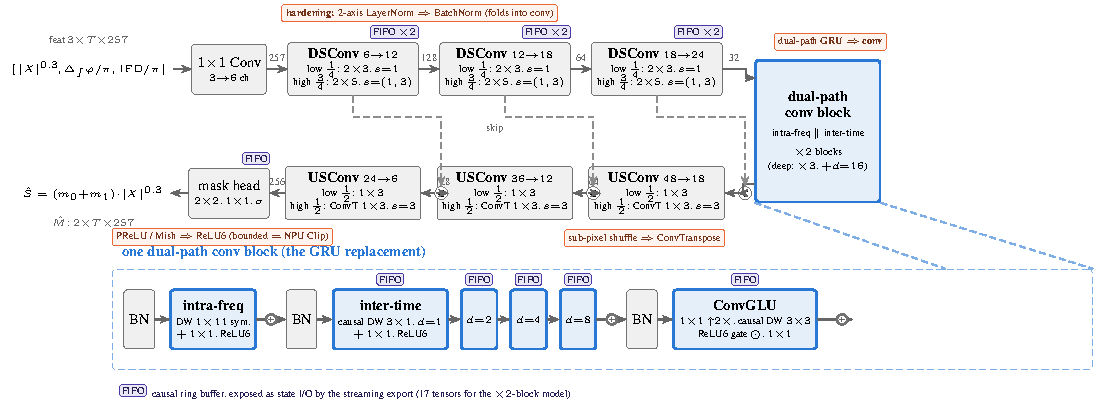
\includegraphics[width=\textwidth]{architecture}
  \caption{The NPU-hardened LiSenNet, drawn as a \emph{diff} against the
  original architecture (Fig.~1 of~\cite{yan2024lisennet}; same layout and
  notation). Green blocks are unchanged; blue blocks are the NPU
  replacements, with orange tags naming what they replace (and globally:
  LayerNorm~$\Rightarrow$~BatchNorm, which folds into the convolutions;
  PReLU/Mish~$\Rightarrow$~ReLU6; Sec.~\ref{ssec:hardening}). The ghosted
  Griffin-Lim refinement is dropped at deployment in favor of the noisy
  phase. (b)~expands the dual-path \emph{conv} (DPC) module that replaces the
  dual-path recurrent (DPR) module --- unlike the DPR, it needs no
  batch-merging reshapes, which are themselves NPU-unmappable
  (Sec.~\ref{sec:background}). Violet chips mark the causal ring buffers the
  streaming export exposes as explicit state I/O (Sec.~\ref{ssec:deploy}).}
  \label{fig:arch}
\end{figure*}

% ===========================================================================
\section{LiSenNet and the NPU gap}
\label{sec:background}

\textbf{LiSenNet}~\cite{yan2024lisennet} is a $\sim$37\,k-parameter
magnitude-masking enhancer. A three-channel input
$[\,|X|^{0.3},\, \Delta_f\varphi/\pi,\, \mathrm{IFD}/\pi\,]$ (power-compressed
magnitude, group delay, and instantaneous-frequency deviation) feeds a
sub-band U-Net encoder, a dual-path recurrent (DPR) bottleneck
--- a bidirectional GRU over frequency and a unidirectional GRU over time ---
and a mask decoder producing two additive multiplicative gains on the noisy
magnitude. Phase is not modeled: the enhanced magnitude is combined with the
noisy phase, optionally refined by two Griffin-Lim
iterations~\cite{griffin1984gl} offline. Trained with the CMGAN
recipe~\cite{cao2022cmgan} (complex + magnitude + MetricGAN~\cite{fu2021metricganplus}
losses) on VoiceBank-DEMAND~\cite{valentini2016vbd}, our reproduction reaches
wideband PESQ~\cite{itu2007pesq} 3.006 (paper: $\sim$3.07).

\textbf{The target NPU.} Neural-ART is an int8-only convolution/matmul
engine. The compiler partitions the graph into \emph{epochs} that run on the
accelerator (HW), on the Cortex-M55 (SW), or cooperatively (hybrid); every
operator outside the supported vocabulary silently becomes M55 software.
Stock LiSenNet does not even compile: the DPR's two-axis LayerNorm has a 2-D
affine the hardware's per-channel normalization cannot express, and the
frequency-axis GRU is unimportable in both its fused and unrolled forms
(a 32-step bidirectional recurrence explodes to $\sim$850 slices). Beyond
these hard blockers, three further primitives break int8 codegen:
per-channel PReLU/Mish activations, the sub-pixel upsampler (its
view--permute--view emits rank-5 tensors, which segfault the compiler), and
--- for the streaming export --- a \texttt{Pad} operator form discussed in
Sec.~\ref{ssec:deploy}.\footnote{The last is a pure toolchain defect:
\texttt{F.pad} exports \texttt{Pad(data, pads, "")} with a present-but-empty
optional input, which crashes the Neural-ART backend inside multi-branch
subgraphs. We strip the empty slot at export time; the transform is
bit-exact.}

% ===========================================================================
\section{NPU-friendly redesign}
\label{sec:redesign}


\subsection{Dual-path convolutions replace the DPR}
\label{ssec:dpc}

We keep LiSenNet's macro-structure --- sub-band encoder
($257\!\to\!128\!\to\!64\!\to\!32$ frequency bins; each stage splits the band
into a low quarter processed at stride 1 and a high three-quarters
downsampled by 3), U-Net skip connections, and the two-gain mask head --- and
replace only the bottleneck. The \emph{intra-frequency} GRU becomes a
symmetric depthwise convolution over frequency (kernel 11) followed by a
pointwise mix: frequency is fully available at each frame, so bidirectional
context needs no recurrence. The \emph{inter-time} GRU becomes a stack of
causal dilated depthwise convolutions (kernel 3, dilations $1,2,4,8$, with a
convolutional GLU~\cite{luo2019convtasnet} after each block), giving a
bounded receptive field of 68 frames ($\approx$1.1\,s) in the base
configuration and 196 frames ($\approx$3.1\,s) in the deeper one (3 blocks,
dilations up to 16). The exported graph contains no GRU and no
LayerNormalization node.

\subsection{Hardening the primitives}
\label{ssec:hardening}

Three further swaps make every operator HW-mappable \emph{and}, as
Sec.~\ref{ssec:quant} shows, quantization-friendly:
(1)~\textbf{norm}: the per-frame two-axis LayerNorm becomes per-channel
BatchNorm, which folds into the preceding convolution at export;
(2)~\textbf{activation}: PReLU/Mish become ReLU6 --- a bounded clip that both
caps every activation's dynamic range for the quantizer \emph{and} disappears
at int8, since a $[0,6]$ clamp folds into the requantization range (the
deployed graph contains no explicit activation op and no extra software epoch;
Sec.~\ref{ssec:silicon});
(3)~\textbf{upsampling}: the sub-pixel shuffle becomes a plain
$1\times3$/stride-3 transposed convolution (4-D tensors only, $\sim$3$\times$
fewer decoder MACs). Retrained from scratch with the unchanged CMGAN recipe,
the hardened model \emph{matches} the GRU reference at the right capacity
(Table~\ref{tab:quality}): capacity is non-monotonic (36\,k $>$ 49\,k), and
clipping even helps training in the deep configuration.

\subsection{Two deployment graphs}
\label{ssec:deploy}

The model is causal, so frame $n$ needs only the previous $\mathrm{RF}$
frames. That admits two exports at the \emph{same} one-hop latency, and which
one is cheaper on an NPU is not obvious \emph{a priori}.

The \textbf{FIFO streaming} graph exposes every causal ring buffer as an
explicit graph input/output (17 state tensors for the base model, 25 for the
deep one) and runs one frame per call with no recompute. It compiles only
after the \texttt{Pad} normalization of Sec.~\ref{sec:background}; its states
quantize with a calibration loader that propagates \emph{real} state
trajectories through the trained model rather than zeros.

The \textbf{stateless RF-window} graph deletes the state machinery entirely:
the host keeps a rolling $(\mathrm{RF}{+}T)$-frame input window, the graph
runs the offline causal model over it and emits the last $T$ mask frames. At
$T{=}1$ it has the same 16\,ms latency as streaming and is \emph{bit-exact} to
the offline model once the window holds real history (FP32 cosine
$1.0000001$, max deviation $7\cdot10^{-7}$; the first $\mathrm{RF}$ frames run
on zero history --- the same warm-up a FIFO has). It trades
$\mathrm{RF}$-fold recompute for zero state plumbing, which is tempting on an
accelerator whose Slice/Concat state ops never map to pure hardware. Larger
$T$ amortizes that recompute but re-introduces $T$ frames of block latency.
Sec.~\ref{ssec:silicon} settles the trade on silicon.

\subsection{Quantization: finding and fixing the int8 loss}
\label{ssec:quant}

All deployments use signed per-channel QDQ post-training quantization (PTQ)
with percentile calibration; the NPU rejects unsigned activations.
Quantization-aware fine-tuning with a reconstruction loss \emph{regressed}
($-0.085$ PESQ): it pulls weights off the MetricGAN optimum, and with a
$-0.016$ PTQ gap there is nothing to recover, so PTQ is the deployment path.
Extending the receptive field, however, exposed a real PTQ problem: the
long-RF variants gain up to $+0.056$ FP32 but lose $\approx0.08$ to int8. A
selective-quantization scan --- one node group kept FP32 at a time, under
\emph{seeded} calibration crops, since calibration-draw noise alone spans
$\pm0.04$ --- localizes the loss: keeping the \emph{decoder} FP32 recovers
$+0.052$ of the $+0.078$ gap, while every other group, the dilated time stack
included, contributes $\leq+0.010$. The decoder's upsampling path is linear
(no ReLU between skip-concatenations and convolutions), so its activation
range grows unchecked as features enrich with receptive field. Two remedies
compose: ReLU6 bounds every clipped tensor (all-int8 PESQ 3.014), and a
\textbf{hybrid} recipe leaves the decoder's nodes ($\sim$36\% of MACs)
unquantized in the QDQ graph for PESQ 3.052 --- but the float decoder costs
19 software epochs instead of 6, 3.5\,MB of weights and 12.3\,MB of
activations, and measures 34\,ms per frame on the board: \emph{the best
offline recipe is not deployable} (Sec.~\ref{ssec:silicon}). ReLU6, which
reaches 3.014 well inside the real-time budget, is the one that ships.
Mask-level knowledge distillation~\cite{hinton2015kd} from the deep teacher
into the small base architecture is a third option (3.004 all-int8 at
36\,k params).

% ===========================================================================
\section{Experiments}
\label{sec:experiments}

\subsection{Setup}
\label{ssec:setup}

All models train on VoiceBank-DEMAND (16\,kHz)~\cite{valentini2016vbd} with
the CMGAN losses (complex 0.1, magnitude 0.9, adversarial 0.05;
MetricGAN-PESQ discriminator), AdamW ($\beta{=}0.8/0.99$, lr $5{\cdot}10^{-4}$,
decay 0.98), STFT 512/256, 100--140 epochs. PESQ is wideband, on the full
824-utterance test split; \emph{real-time int8} means static-int8 mask
inference combined with the noisy phase (no Griffin-Lim). Deployment uses ST
Edge AI Core 4.0.1~\cite{st2024edgeai} on the STM32N6570-DK; ONNX export and
quantization use ONNX Runtime~\cite{onnxruntime}. On-board latency is the
on-target validation figure (10 runs); the epoch/memory data come from the
compiler report and an on-device per-epoch profiler.

\subsection{Quality}
\label{ssec:quality}

\begin{table}[t]
  \centering
  \caption{VoiceBank-DEMAND quality ladder (full 824-utt test split). RT-int8
  = static int8 + noisy phase, the deployable configuration. RF in frames
  (16\,ms hop). The ``$+$'' rows are cumulative architecture changes on
  ``hardened, 24\,ch'' ($+$\,dilation 16 adds one dilation stage;
  $+$\,3 blocks adds a third dual-path block; relu6-deep swaps ReLU$\to$ReLU6
  at the same shape) --- each is trained from scratch with the same recipe,
  not warm-started from the row above.}
  \label{tab:quality}
  \small
  \begin{tabular}{@{}lrrcc@{}}
    \toprule
    model & params & RF & FP32 & RT-int8 \\
    \midrule
    LiSenNet (GRU, repro.)~\cite{yan2024lisennet} & 36.8\,k & $\infty$ & 3.006 & 2.930 \\
    dual-path conv (unhardened)        & 41.1\,k & 68  & 2.970 & 2.855 \\
    \midrule
    hardened, 20 ch                    & 25.7\,k & 68  & 2.895 & 2.853 \\
    hardened, 24 ch                    & 36.3\,k & 68  & 3.013 & 2.998 \\
    hardened, 28 ch                    & 48.7\,k & 68  & 2.927 & 2.867 \\
    \midrule
    ~+ dilation 16                     & 37.7\,k & 132 & 3.034 & 2.954 \\
    ~+ 3 blocks (deep)                 & 46.2\,k & 196 & 3.069 & 2.985 \\
    \textbf{relu6-deep} (all-int8)     & 46.2\,k & 196 & \textbf{3.084} & \textbf{3.014} \\
    \quad w/ FP32 decoder (hybrid)     & 46.2\,k & 196 & 3.084 & \textbf{3.052} \\
    \bottomrule
  \end{tabular}
\end{table}

Table~\ref{tab:quality} tells the story in three acts. Hardening costs
nothing at the right width --- 24 channels matches the GRU reference in FP32
--- and \emph{fixes quantization}: the PTQ drop shrinks from $-0.115$
(unhardened) to $-0.016$, attributable to BatchNorm folding, parameter-free
bounded activations, and signed per-channel quantization rather than
capacity. Receptive field buys FP32 quality almost linearly
($\approx+0.02$ per doubling) but PTQ initially takes it all back
($-0.080$/$-0.084$); the decoder-localized fixes of Sec.~\ref{ssec:quant}
then unlock it. Net effect across the study: deployable real-time PESQ rises
from 2.855 to \textbf{3.052} ($+0.122$ over the GRU reference), with every
operator NPU-safe. A second seed reproduces the 24-channel result within
$\pm0.004$.

\subsection{On-device results}
\label{ssec:silicon}

\begin{table*}[t]
  \centering
  \caption{\textbf{On-device cost of every LiSenNet variant}, measured on the
  STM32N6570-DK (Neural-ART @ 1\,GHz, Cortex-M55 @ 800\,MHz), int8, one
  toolchain pass per row (stedgeai 4.0.1 $\to$ RAM firmware $\to$ on-target
  validation). Blocks (a) and (b) are the \emph{same} 16\,ms algorithmic
  latency and differ only in how the causal context is carried --- explicit
  FIFO state vs.\ recomputing the receptive-field window; (c) amortizes that
  window over a 64-frame emit block and is a throughput mode. ms/frame is per
  \emph{emitted} frame; RTF = ms/frame $\div$ 16\,ms. RF in frames; PESQ is
  wideband on the full 824-utterance split, as in Table~\ref{tab:quality}.}
  \label{tab:silicon}
  \small
  \setlength{\tabcolsep}{4.5pt}
  % table2_body.tex is GENERATED from the measured sweep (compile reports +
  % on-target validate); regenerate rather than hand-edit.
    \begin{tabular}{@{}lrrrrrrr@{}}
    \toprule
    deployment & params & RF & MAC/frame & weights & ms/frame & RTF & PESQ \\
    \midrule
    \multicolumn{8}{@{}l}{\textbf{(a) FIFO streaming} --- one frame in, one out; \textbf{16\,ms} algorithmic latency} \\
    hardened, 20\,ch$^\ddagger$ & 25.7\,k & 68 & 0.92\,M & 35\,KB & 2.59 & 0.16 & --- \\
    hardened, 24\,ch & 36.3\,k & 68 & 1.30\,M & 47\,KB & 2.79 & 0.17 & 2.963 \\
    hardened, 28\,ch$^\ddagger$ & 48.7\,k & 68 & 1.75\,M & 62\,KB & 3.15 & 0.20 & --- \\
    \quad+ dilation 16$^\ddagger$ & 37.7\,k & 132 & 1.38\,M & 50\,KB & 3.63 & 0.23 & --- \\
    \quad+ 3 blocks (deep)$^\ddagger$ & 46.2\,k & 196 & 1.69\,M & 62\,KB & 4.88 & 0.30 & --- \\
    \textbf{relu6-deep} & 46.2\,k & 196 & 1.66\,M & 61\,KB & \textbf{4.83} & \textbf{0.30} & 3.013 \\
    \midrule
    \multicolumn{8}{@{}l}{\textbf{(b) stateless RF-window}, $T{=}1$ --- no state, recomputes the receptive field every frame; same \textbf{16\,ms} latency} \\
    hardened, 20\,ch$^\dagger$$^\ddagger$ & 25.7\,k & 68 & 66.55\,M & 406\,KB & 29.93 & 1.87 & 2.853 \\
    hardened, 24\,ch$^\dagger$ & 36.3\,k & 68 & 92.89\,M & 492\,KB & 32.81 & 2.05 & 2.998 \\
    hardened, 28\,ch$^\dagger$$^\ddagger$ & 48.7\,k & 68 & 123.76\,M & 580\,KB & 40.01 & 2.50 & 2.867 \\
    \quad+ dilation 16$^\dagger$$^\ddagger$ & 37.7\,k & 132 & 185.02\,M & 710\,KB & 74.72 & 4.67 & 2.954 \\
    \quad+ 3 blocks (deep)$^\dagger$$^\ddagger$ & 46.2\,k & 196 & 336.31\,M & 938\,KB & 127.16 & 7.95 & 2.985 \\
    \textbf{relu6-deep}$^\dagger$ & 46.2\,k & 196 & 335.75\,M & 938\,KB & 119.86 & 7.49 & 3.014 \\
    \midrule
    \multicolumn{8}{@{}l}{\textbf{(c) RF-window amortized}, $T{=}64$ --- throughput mode, \textbf{1.02\,s} block latency (not real-time \emph{latency})} \\
    hardened, 24\,ch & 36.3\,k & 68 & 2.78\,M & 492\,KB & 1.15 & 0.07 & 2.998 \\
    \textbf{relu6-deep} & 46.2\,k & 196 & 6.92\,M & 938\,KB & 3.09 & 0.19 & 3.014 \\
    relu6-deep, hybrid dec.$^\dagger$ & 46.2\,k & 196 & 6.91\,M & 3.51\,MB & 33.99 & 2.12 & 3.052 \\
    \midrule
    \multicolumn{8}{@{}l}{\emph{other model families --- same board, same flow, FIFO streaming}} \\
    ConvFSENet~\cite{luo2019convtasnet} & 1.45\,M & --- & 1.47\,M & 1.40\,MB & 4.40 & 0.28 & 2.911 \\
    NSNet2 monarch\_full~\cite{dao2022monarch} & 0.36\,M & --- & --- & 0.72\,MB & 2.13 & 0.13 & 2.848 \\
    NSNet2 monarch\_8~\cite{dao2022monarch} & 0.36\,M & --- & 0.39\,M & 0.37\,MB & 2.89 & 0.18 & 2.826 \\
    NSNet2 dense~\cite{braun2020nsnet2}$^\dagger$ & 2.78\,M & --- & --- & 2.70\,MB & 22.94 & 1.43 & 2.833 \\
    \bottomrule
  \end{tabular}
\\[2pt]
  {\footnotesize $^\dagger$exceeds the 16\,ms budget: not real-time.\quad
  $^\ddagger$latency measured on the compiled graph of that architecture with
  re-initialized weights (no trained checkpoint at hand); the graph --- and
  hence the latency --- is identical, and PESQ is the host-measured value from
  Table~\ref{tab:quality}.}
\end{table*}

We deployed \emph{every} hardened variant, in both graph forms, through one
toolchain pass each (Table~\ref{tab:silicon}). Four observations.

\textbf{The design space is real-time, streaming, end to end.} Every variant
runs frame-by-frame within the 16\,ms budget: 2.59\,ms (20\,ch) to 4.88\,ms
(3 blocks, RF 196), i.e.\ RTF 0.16--0.31, with weights (35--62\,KB) and
activations ($\leq$304\,KB) entirely in on-chip NPU RAM. Latency grows
sub-linearly with capacity and receptive field --- doubling RF from 68 to 196
frames costs $1.7\times$ the frame time --- so the quality knobs of
Sec.~\ref{ssec:quant} are affordable on this silicon. The deployed model,
\textbf{relu6-deep, streams at 4.83\,ms/frame (RTF 0.30) at PESQ 3.013}: the
best-quality real-time streaming enhancer on this board, ahead of ConvFSENet
(2.911 at 4.40\,ms) and the sparse NSNet2 variants (2.85 at 2.13\,ms), and at
true one-hop latency. On-target outputs track the host int8 reference at
cosine 0.998.

\textbf{Deleting the FIFO is a trap.} At the same 16\,ms latency, the stateless
RF-window (block~b) is \textbf{11.6--26$\times$ slower} and misses real time for
\emph{every} variant. Not because it maps badly --- the opposite: with no
Slice/Concat state ops it sustains $6\text{--}8\times$ higher utilization
(2.2--3.1 vs.\ 0.34--0.56\,GMAC/s), confirming the streaming graph is
launch/state-bound. But it recomputes the whole receptive field every frame
($70\times$ the MACs at RF~68, $200\times$ at RF~196), and that gain cannot pay
that bill; amortizing (block~c) restores real time only by trading back
latency. \emph{The FIFO dominates on both axes}, which is what makes the
\texttt{Pad} export fix (Sec.~\ref{sec:background}) load-bearing: without it the
only NPU-mappable graph was the window, and this model would not be real-time.

\textbf{The FP32 \emph{decoder} is what fails to ship --- not ReLU6}, which
folds into the quantization for free (6 software epochs, like every pure-int8
variant). The \emph{hybrid} recipe (FP32 decoder, PESQ 3.052) is the one that
does not run: its float decoder pulls 19 epochs onto the Cortex-M55 and
measures \textbf{34\,ms/frame, RTF 2.1} --- past the budget.
Sec.~\ref{ssec:quant}'s activation clipping recovers most of that quality
(3.014) \emph{inside} it, and is the deployable answer.

\textbf{The frame cost is launch-bound, not compute-bound.} Per-epoch
profiling of the 24-channel streaming graph shows the NPU core busy for only
0.72\,ms of 2.79\,ms (26\%); the floor is the launch and state-plumbing
overhead of its 131 epochs --- the same regime as the ConvFSENet baseline, and
why the windowed graphs amortize better. (Re-measuring the 24-channel rows
eleven days apart reproduced 2.789 vs.\ 2.791\,ms, so the comparisons are
inside run-to-run noise.)

\subsection{Should the time axis be a convolution at all?}
\label{ssec:recurrence}

We replaced \emph{both} GRUs with convolutions, but only the intra-frequency
one is uncontroversial (bidirectional over an axis fully available per frame).
The inter-time conv instead approximates recurrence's unbounded memory with a
dilated FIFO. A \emph{hybrid} bottleneck --- conv on frequency, GRU on time ---
isolates that single choice at matched parameters (Table~\ref{tab:recurrence}).
Recurrence is not un-deployable: at $t{=}1$ a GRU step is a set of $1\times1$
convolutions with the hidden state as one more state tensor, so it exports with
\emph{zero} GRU ops, maps to hardware (6 software epochs, like every variant),
and runs \textbf{1.5--2.2$\times$ faster with 4--6$\times$ less state} than the
FIFO --- state machinery, not arithmetic, is the streaming graph's cost.

\begin{table}[t]
  \centering
  \caption{Recurrence vs.\ convolution on the \emph{time} axis, at matched
  parameters (conv-on-frequency held fixed). Streaming int8, on the
  STM32N6570-DK; PESQ on the full test split. GRU rows have $\mathrm{RF}=\infty$.}
  \label{tab:recurrence}
  \small
  \setlength{\tabcolsep}{4pt}
  \begin{tabular}{@{}llrrrr@{}}
    \toprule
    time mixer & RF & ms/frame & state & FP32 & int8 \\
    \midrule
    conv (FIFO), nc24     &  68 & 2.79 & 147\,KiB & \textbf{3.013} & \textbf{2.963} \\
    \textbf{GRU}, nc24     & $\infty$ & \textbf{1.82} & \textbf{40\,KiB} & 2.953 & 2.867 \\
    \midrule
    conv (FIFO), deep     & 196 & 4.82 & 307\,KiB & \textbf{3.084} & \textbf{3.013} \\
    \textbf{GRU}, deep     & $\infty$ & \textbf{2.18} & \textbf{52\,KiB} & 3.073 & 2.975 \\
    \bottomrule
  \end{tabular}
\end{table}

The quality trade is \emph{receptive-field-dependent}, which is the point. At
RF~68 the GRU loses (Table~\ref{tab:recurrence}): 68 frames of bounded context
already suffice, and its recursive $\tanh/\sigma$ state --- unbounded, with no
ReLU to clamp it --- quantizes far worse (PTQ drop $-0.104$ vs.\ the conv's
$-0.015$, the Sec.~\ref{ssec:quant} effect on a recurrence). At RF~196 the gap
essentially closes: the FP32 $-0.011$ is within the seed noise of
Sec.~\ref{ssec:quality} and the int8 drop is now comparable, not $7\times$
worse --- unbounded recurrence becomes competitive exactly where the FIFO
spends the most state to fake it. What the conv keeps at every RF is a
\emph{certifiable} recovery guarantee: its state \emph{is} the last
$\mathrm{RF}$ inputs, so after a glitch two streams re-converge to identical
output within $\mathrm{RF}$ frames (measured: 68, 196) --- a bound the IIR GRU
cannot offer. The honest summary is \emph{efficiency vs.\ certifiability}:
convolution is the safe default we ship; recurrence-on-time is the better bet
at long receptive fields, matching quality at half the latency and a sixth of
the state, where the recovery guarantee can be forgone.

% ===========================================================================
\section{Conclusion}
\label{sec:conclusion}

We turned a GRU-centric lightweight enhancer into an NPU-native one and showed
the redesign is not a compromise: the convolutional dual-path bottleneck
matches the recurrent original in FP32, the hardening the hardware demands is
what makes int8 nearly free, and the one place quantization still hurts --- the
linear decoder --- is diagnosable and repairable with activation clipping
inside the latency budget, where a float decoder is not. The deployed model
streams frame-by-frame at 16\,ms latency, real-time factor 0.30, while
\emph{exceeding} the CPU-oriented original's deployable quality by $+0.083$
PESQ. Along the way, two comparisons at equal latency map the design space:
recompute-in-a-window loses to explicit state by $12\text{--}26\times$, while
recurrence-on-time (once written as convolutions) \emph{beats} the conv+FIFO
on efficiency and ties it on quality at long receptive fields --- state, not
recompute, and a compressed state at that, is what makes this class of model
real-time. We believe the recipe --- re-express recurrence as NPU-native ops,
harden primitives for the int8 vocabulary, and treat quantization robustness
as a design criterion --- transfers beyond this model and accelerator.

% ===========================================================================
\vfill\pagebreak

\bibliographystyle{IEEEbib}
\bibliography{refs}

\end{document}
